\documentclass[journal]{IEEEtran}
\usepackage{amsmath,amssymb,bm}
\usepackage{booktabs,multirow}
\usepackage{graphicx}
\usepackage{url}
\usepackage{cite}
\usepackage{xcolor}
\usepackage{hyperref}
\usepackage{tikz}
\usetikzlibrary{positioning,arrows.meta}
\graphicspath{{figures/}}
\newcommand{\method}{TrustKAN-Climate}
% A placeholder that reaches the PDF is a defect, so leave none that can. This
% stops the build instead of printing a red note a reader might never see.
\newcommand{\todo}[1]{%
  \GenericError{}{Unresolved \string\todo: #1}{}{%
    Resolve it or delete it; the manuscript may not ship a placeholder.}%
}
% Degrees Celsius without a siunitx dependency, so the manuscript builds on a
% bare TeX installation like the artifacts it documents.
\newcommand{\degC}{\ensuremath{^{\circ}}C}

% Quantities quoted in prose, generated from the frozen ledgers so that text and
% tables cannot drift apart. A missing generated file must stop the build rather
% than silently leave every macro it defines undefined, which on a case-sensitive
% filesystem is the difference between a caught error and a wrong manuscript.
\newcommand{\generated}[1]{%
  \IfFileExists{#1}{\input{#1}}{%
    \GenericError{}{Generated input #1 is missing; run the generators or
      scripts/make_paper_bundle.py}{}{No numeric macro may be typed by hand,
      so the build stops instead of proceeding without it.}%
  }%
}
\generated{tables/cet_prose.tex}
\generated{tables/ghcn_frozen_panel.tex}
\generated{tables/cet_derived.tex}
\generated{tables/cet_adaptive.tex}
\generated{tables/cet_dataset.tex}
\generated{tables/cet_rolling.tex}
\generated{tables/cet_curves.tex}
\generated{tables/cet_defect.tex}
\generated{tables/cet_robustness_macros.tex}

\title{A Trustworthy Forecasting Framework That Fails Its Own Tests: A Pre-Registered Evaluation of Reliability-Aware Kolmogorov--Arnold Networks for Climate Forecasting}

\author{Yongxiang Lei,~\IEEEmembership{Member,~IEEE}%
\thanks{Author affiliations, funding acknowledgements, and correspondence details will be finalized before submission.}}

\begin{document}
\maketitle

\begin{abstract}
Trustworthy forecasting is routinely claimed on architectural grounds: a model that emits quantiles, scores distribution shift, and abstains is presented as reliable because it contains machinery for reliability. We tested that reasoning on our own design. \method{} couples a temporal Kolmogorov--Arnold Network (KAN) with quantile prediction, split-conformal calibration, an embedding-shift score, and reliability-based selective forecasting. Before running the headline experiments we froze the datasets, splits, horizons, seeds, comparison family, and calibration constants, and we recorded each claim against the evidence that would be required to support it. On \cetSpanYears{} years of daily Central England Temperature station observations at horizons of 1, 7, 30, and 90 days, with five seeds and nine baselines, the framework fails almost every test it set for itself. It wins none of forty pre-specified paired comparisons under a circular block bootstrap over forecast origins: a plain KAN of matched budget is significantly better at 7, 30, and 90 days, and a transformer is significantly better at all four horizons. Conformal marginal coverage does land on nominal (\coverageLow{}--\coverageHigh{} against \nominalCoverage{}), but this is the split-conformal guarantee and holds for any backbone, while per-origin joint coverage degrades from \jointCoverageOne{} to \jointCoverageNinety{} as lead time grows. The proposed reliability score is beaten by its own interval-width component at every horizon, and it identifies high-error forecasts at chance (AUROC \errorAurocLow{}--\errorAurocHigh{}), so abstaining on half of all origins reduces error by only one to three percent. An eighty-run ablation is more damaging still: replacing the KAN mapping with a budget-matched multilayer perceptron changes RMSE by at most \ablationKanGapMax{}\,\degC{}, so the component that names the architecture contributes nothing measurable. The interpretability that motivates a KAN does not survive either. Retraining every reported run to recover its weights, and accepting only runs that reproduce their ledger RMSE exactly, we find that a given univariate curve denotes nothing stable: correlation between the same curve index in two seeds is \curveMatchedOne{}. The two obvious ways to rescue that number both match their own controls exactly, because the layer's \curveCount{} curves span only \curveRankMax{} effective dimensions. A pre-registered corruption sweep then refutes the robustness claim and diagnoses the rest: the model is the most fragile of its comparison family at every corruption level, and masking recent days stops costing it anything past three days because, of the \robustHistory{} days of history it is configured to receive, only \robustFieldTrust{} reach its readout. We also report an architectural defect found and corrected mid-study, together with the audit that caught it. Three findings survive, and all belong to the conformal wrapper rather than to the proposed method: interval width alone supports useful selective forecasting, improving on no abstention by up to \widthGainNinety{}; adaptive conformal calibration cuts rolling coverage deviation by up to \adaptiveDevDropNinety{} for a width cost of at most \adaptiveWidthCostThirty{}; and pre-registration with checksum-bound artifacts is what converted a publishable-looking result into a refutation. We argue that reliability machinery must be evidenced component by component against its own ablations rather than credited to the architecture that contains it.
\end{abstract}

\begin{IEEEkeywords}
Kolmogorov--Arnold networks, climate forecasting, trustworthy artificial intelligence, uncertainty quantification, conformal prediction, distribution shift, selective prediction, interpretability.
\end{IEEEkeywords}

\section{Introduction}
\label{sec:introduction}

Data-driven climate and weather forecasting has benefited from rapid progress in deep temporal models, including recurrent networks, attention-based architectures, state-space models, and more recently Kolmogorov--Arnold Networks (KANs). However, improved point accuracy alone is insufficient for scientific and operational use. Forecast systems are deployed across changing regimes, imperfect observations, nonstationary seasonal patterns, and distribution shifts that can invalidate assumptions learned from historical data. Under these conditions, a model should not only predict accurately but also reveal relevant nonlinear relationships, quantify predictive uncertainty, detect when the current regime differs from calibration experience, and reduce reliance on predictions that are likely to be unreliable.

KAN-based predictors are particularly attractive because learnable univariate functions can expose nonlinear response structure more directly than conventional multilayer perceptrons. Yet the presence of KAN layers does not by itself establish trustworthy forecasting. Three gaps remain important. First, interpretability must be demonstrated through stable, inspectable functional relationships rather than asserted from architecture alone. Second, probabilistic uncertainty must be empirically calibrated, including under temporal shift. Third, model confidence should be connected to actionable reliability, for example through selective prediction that trades forecast coverage against risk.

This work develops \method, a unified framework for interpretable and reliability-aware climate forecasting. The proposed system combines a temporal KAN representation with point and quantile prediction, conformal calibration, representation-level shift assessment, and a reliability score used for selective prediction. A dedicated calibration partition is retained between model validation and final testing so that conformal correction and abstention thresholds are selected without using final test outcomes.

The intended contributions are as follows:
\begin{itemize}
    \item We develop a temporal KAN forecasting architecture that preserves nonlinear functional structure while modelling temporal dependence for multi-horizon climate prediction.
    \item We integrate quantile prediction with static, rolling, and adaptive conformal calibration to evaluate whether predictive coverage can be maintained as data distributions evolve.
    \item We formulate reliability using uncertainty width and representation-shift evidence, and evaluate whether the resulting score is associated with realized forecast error rather than treating confidence as self-validating.
    \item We introduce reliability-based selective forecasting and evaluate the risk--coverage trade-off, including whether abstention removes disproportionately high-error predictions.
    \item We design a multi-dataset, multi-horizon evaluation protocol with strong classical, neural, KAN, and state-space baselines, multiple random seeds, statistical comparison, robustness analysis, computational evaluation, and explicit failure-case reporting.
\end{itemize}

The paper is organized as follows. Section~\ref{sec:related} reviews relevant work. Section~\ref{sec:method} presents \method. Section~\ref{sec:experiments} defines the datasets and evaluation protocol. Section~\ref{sec:results} reports empirical results, followed by discussion and limitations in Section~\ref{sec:discussion}.

\section{Related Work}
\label{sec:related}

\subsection{Data-Driven Time-Series Forecasting}
Modern time-series forecasting increasingly relies on deep sequence models in addition to classical statistical and tree-based methods. Transformer-based forecasting has been strengthened by patching and channel-independent processing, as exemplified by PatchTST \cite{nie2022patchtst}. State-space sequence models provide another route to long-context modeling: Mamba introduces input-dependent selective state-space dynamics with linear sequence-length scaling \cite{gu2023mamba}. These model families are why the frozen comparison set in this study includes attention-based and convolutional temporal baselines, although the specific published architectures cited here are not themselves among them. Predictive skill alone, in any case, does not establish whether a forecast should be trusted under non-stationarity.

\subsection{Kolmogorov--Arnold Networks for Temporal Prediction}
Kolmogorov--Arnold Networks (KANs) replace the fixed scalar nonlinearities of conventional multilayer perceptrons with learnable univariate functions on edges, yielding a functional representation that can be visualized and inspected \cite{liu2025kan}. Early work applying KANs to time-series analysis reported competitive forecasting performance with compact parameterizations \cite{vacarubio2024kan}. These developments motivate KANs as an interpretable-by-design forecasting backbone. The present study asks a distinct question: whether a temporal KAN representation can also provide useful evidence about forecast reliability under temporal and distributional shift. Accordingly, interpretability is evaluated through functional stability rather than assumed from architecture alone.

\subsection{Conformal Uncertainty Quantification for Time Series}
Conformal prediction provides a model-agnostic mechanism for calibrating predictive sets from empirical nonconformity scores. Conformalized quantile regression combines learned conditional quantiles with conformal calibration to improve interval adaptivity while retaining marginal coverage guarantees under the corresponding assumptions \cite{romano2019cqr}. Weighted conformal methods have also been developed for covariate shift \cite{tibshirani2019covariate}. For sequential data, conformal time-series forecasting extends inductive conformal ideas to multi-horizon forecasting \cite{stankeviciute2021conformal}, while Adaptive Conformal Inference updates the effective miscoverage level online to address changing distributions \cite{gibbs2021adaptive}. Subsequent work studied adaptive conformal prediction specifically for dependent time series \cite{zaffran2022adaptive}, and control-inspired conformal updates have further targeted systematic temporal errors and distribution shifts \cite{angelopoulos2023pid}. These methods motivate our comparison of static, rolling, and adaptive calibration.

\subsection{Distribution Shift, Reliability, and Selective Prediction}
Selective prediction allows a model to abstain on low-confidence samples, explicitly trading prediction coverage for reduced risk \cite{geifman2017selective}. SelectiveNet further showed that rejection can be incorporated directly into deep models and evaluated through risk--coverage behaviour \cite{geifman2019selectivenet}. Distribution-shift monitoring provides a complementary capability by detecting deviations from a reference operating regime; recent work has connected shift detection with selective-prediction principles in streaming settings \cite{barshalom2023shift}. In \method{}, interval width and representation shift are treated as candidate evidence sources. Crucially, these signals are not assumed to measure reliability: they must demonstrate association with realized forecast error and improved risk--coverage trade-offs on held-out data, and the fusion weight that combines them is selected on the calibration partition rather than frozen in advance.

\section{Methodology}
\label{sec:method}

\subsection{Problem Formulation}
Let $\mathbf{x}_t\in\mathbb{R}^{d}$ denote the climate or weather variables observed at time $t$. Given a history window of length $L$, the forecasting task is to estimate a future target vector $\mathbf{y}_{t+1:t+H}$ over horizon $H$. We seek not only a point forecast $\hat{\mathbf{y}}$ but also a reliability characterization that supports calibrated intervals and selective use of the prediction.

\subsection{Temporal KAN Representation}
The proposed model first maps the input sequence through a temporal encoder and then through a KAN-style nonlinear representation. For a hidden vector $\mathbf{z}$, the KAN mapping is represented as a sum of learnable univariate functions across input dimensions,
\begin{equation}
\mathbf{h}=\mathbf{b}(\mathbf{z})+\sum_j \boldsymbol{\phi}_j(z_j),
\end{equation}
where the current implementation parameterizes $\boldsymbol{\phi}_j$ using Gaussian radial basis expansions. This design preserves inspectable nonlinear functions while allowing the temporal encoder to capture local temporal dependencies.

\subsection{Point and Quantile Forecasting}
The encoded representation is pooled to a fixed-dimensional embedding $\mathbf{e}$. A point head predicts $\hat{\mathbf{y}}$, while a quantile head predicts lower, median, and upper conditional quantiles. Training combines point mean-squared error and quantile pinball loss,
\begin{equation}
\mathcal{L}=\mathcal{L}_{\mathrm{MSE}}+\lambda_q\mathcal{L}_{\mathrm{quantile}}.
\end{equation}
The weighting $\lambda_q$ is treated as a configurable hyperparameter and must be tuned using training/validation data only.

\subsection{Conformal Calibration}
Let $[\hat{\ell}_i,\hat{u}_i]$ denote the model interval for a calibration sample with target $y_i$. The nonconformity score is
\begin{equation}
s_i=\max\{\hat{\ell}_i-y_i,\; y_i-\hat{u}_i,\;0\}.
\end{equation}
A finite-sample conformal radius is obtained from an empirical quantile of the calibration scores and added symmetrically to the predicted interval. We compare static split conformal calibration with rolling and adaptive variants. In the sequential variants, the label for the current time step is incorporated only after its interval has been issued.

\subsection{Distribution-Shift Evidence}
The model embedding $\mathbf{e}$ is used to construct a reference distribution from calibration samples. A Mahalanobis-type distance provides one representation-shift score. This score is converted to a reliability component relative to the empirical calibration distribution. The design is deliberately modular so that representation shift can be removed in controlled ablations.

\subsection{Reliability Fusion}
Two principal evidence sources are considered: normalized prediction-interval width and representation-shift evidence. Let $r_{\mathrm{width}}$ and $r_{\mathrm{shift}}$ denote reliability values in $[0,1]$. The default fusion is a weighted combination,
\begin{equation}
r=w_1r_{\mathrm{width}}+w_2r_{\mathrm{shift}},\qquad w_1+w_2=1.
\end{equation}
The weights and decision threshold are selected from calibration data only. Reliability is subsequently validated by measuring its association with realized forecast error and by risk--coverage analysis.

\subsection{Selective Forecasting}
Given a reliability threshold $\tau$, a forecast is accepted if $r\geq\tau$ and otherwise abstained. For different thresholds, the retained fraction defines coverage and the prediction error among retained samples defines risk. The resulting risk--coverage curve and its area quantify whether reliability-based abstention preferentially removes high-error predictions.

\subsection{Interpretability and Explanation Stability}
KAN univariate response functions are inspected across random seeds, time periods, and perturbed inputs. Stability is evaluated through function correlation and normalized distance metrics. Importantly, explanation stability is considered a core reliability component only if ablation experiments show incremental predictive value for realized error or selective risk; otherwise it is reported solely as an interpretability diagnostic.

\section{Experimental Setup}
\label{sec:experiments}

\subsection{Datasets}
The study is designed around four complementary climate/weather sources: Central England Temperature (CET), NOAA/NCEI GHCN-Daily station observations, Jena weather-station measurements, and ERA5 reanalysis. CET provides continuity with prior climate KAN work; GHCN-Daily evaluates station-level geographic generalization; Jena provides high-frequency multivariate observations; and ERA5 supports reanalysis-based multivariate and distribution-shift experiments. Exact station choices, variables, date ranges, units, missing-data rules, licenses, and download procedures must be frozen before headline experiments. \todo{Populate Table~\ref{tab:datasets} only after dataset metadata are finalized.}

\begin{table}[t]
\centering
\caption{Dataset characteristics. All entries must be generated from finalized dataset metadata.}
\label{tab:datasets}
\begin{tabular}{lcccc}
\toprule
Dataset & Resolution & Variables & Period & Samples \\
\midrule
CET & \todo{daily} & \todo{} & \todo{} & \todo{} \\
GHCN-Daily & \todo{} & \todo{} & \todo{} & \todo{} \\
Jena & \todo{} & \todo{} & \todo{} & \todo{} \\
ERA5 & \todo{} & \todo{} & \todo{} & \todo{} \\
\bottomrule
\end{tabular}
\end{table}

\subsection{Chronological Splitting and Leakage Prevention}
All time series are split chronologically into training, validation, calibration, and final test regions. Normalization parameters are estimated from training observations only. Windowed samples are assigned according to forecast-target origin, and windows whose forecast target crosses a split boundary are excluded. Hyperparameter selection uses training and validation data; conformal correction and reliability thresholds use calibration data; the final test set is reserved exclusively for evaluation.

\subsection{Forecasting Tasks}
Experiments include multiple forecast horizons selected according to each dataset's temporal resolution. The CET development benchmark currently considers 1-, 7-, 30-, and 90-step horizons. Equivalent horizon sets for other datasets will be specified before final experiments so that comparisons are meaningful within each temporal resolution.

\subsection{Baselines}
The benchmark includes persistence and classical machine-learning models, recurrent networks, temporal convolution, Transformer and state-space sequence models, a standard KAN baseline, a Tem$^2$-KAN reference implementation, and the proposed \method. Optional models are reported as failed/unavailable rather than silently removed if dependencies or execution fail. Hyperparameter tuning effort should be comparable across major learned baselines.

\subsection{Evaluation Metrics}
Deterministic forecasting is evaluated using MAE and RMSE in physical target units. Probabilistic forecasting uses empirical interval coverage, mean prediction-interval width, and interval/calibration scores where supported. Reliability is evaluated using reliability--error correlation, large-error detection AUROC/AUPRC, risk--coverage curves, AURC, retained-sample error, and abstention rate. Efficiency analysis reports parameter count, training time, inference latency, and memory where measurable.

\subsection{Statistical Analysis}
Headline neural comparisons use at least five independent random seeds. Paired comparisons are computed from predictions at identical forecast origins and timestamps. Because adjacent and multi-horizon windows overlap, primary confidence intervals for MAE and RMSE differences use a circular moving-block bootstrap over forecast origins, keeping all horizon elements from each origin together. Block length is fixed before final comparison and is at least the forecast-horizon width. Origin-level Wilcoxon tests and paired standardized mean differences are reported only as sensitivity analyses because they do not model serial dependence. Holm correction is applied to each pre-specified primary comparison family; exploratory families may additionally report Benjamini--Hochberg correction. Statistical evidence is interpreted together with effect magnitude and practical relevance rather than as a binary criterion.

\subsection{Robustness and Shift Protocols}
Robustness experiments include sensor noise, missing inputs, temporal regime shift, and extreme-event subsets. Adaptive/rolling conformal experiments evaluate coverage through time rather than only as an aggregate. Any synthetic corruption level or shift definition must be fixed before examining final model rankings.

\section{Results}
\label{sec:results}

This section must be populated only from machine-readable experiment outputs. Numerical values should not be typed manually into the manuscript.

\subsection{Deterministic Forecasting}
\todo{Insert generated multi-dataset, multi-horizon comparison table. Discuss mean$\pm$std performance, not only the best single run. Report cases where TrustKAN does not rank first.}

\IfFileExists{tables/benchmark_summary.tex}{\input{tables/benchmark_summary.tex}}{}

\subsection{Probabilistic Forecasting and Calibration}
\todo{Insert static conformal and quantile-forecast results: empirical coverage, interval width, interval score, and calibration deviation. Compare static, rolling, and adaptive calibration.}

\subsection{Adaptive Conformal Performance under Drift}
\todo{Report rolling coverage trajectories and interval-width trade-offs under temporal drift. Quantify whether adaptive calibration improves coverage stability and whether it pays for this through excessive interval expansion.}

\begin{figure}[t]
\centering
\IfFileExists{figures/rolling_coverage.pdf}{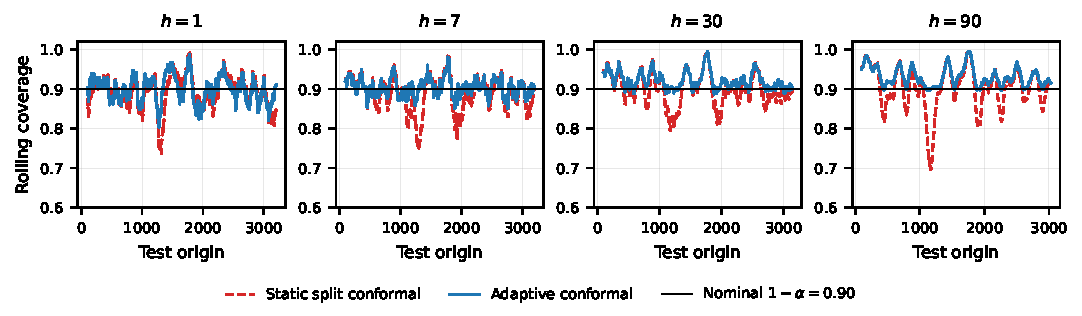
\includegraphics[width=\columnwidth]{rolling_coverage.pdf}}{\fbox{\parbox{0.9\columnwidth}{\centering Rolling coverage figure will be generated from experiment outputs.}}}
\caption{Rolling empirical coverage under static, rolling, and adaptive conformal calibration.}
\label{fig:rollingcoverage}
\end{figure}

\subsection{Reliability--Error Association}
\todo{Report Spearman/Pearson association, reliability-bin errors, and AUROC/AUPRC for identifying high-error predictions. A reliability score that does not predict realized error should not be presented as a core contribution.}

\begin{figure}[t]
\centering
\IfFileExists{figures/reliability_vs_error.pdf}{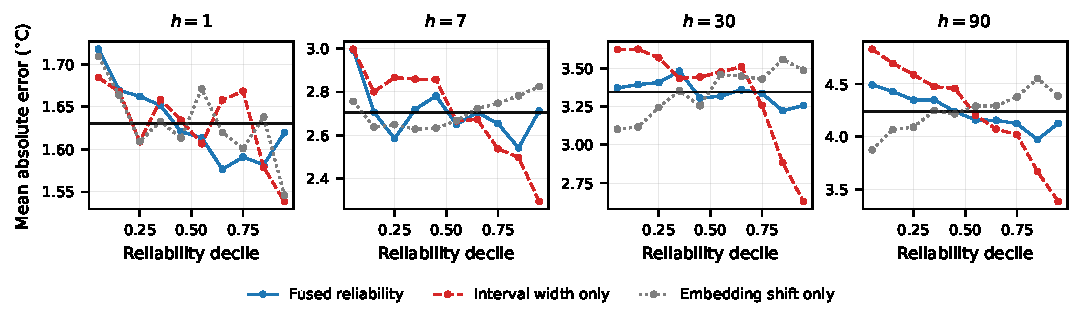
\includegraphics[width=\columnwidth]{reliability_vs_error.pdf}}{\fbox{\parbox{0.9\columnwidth}{\centering Reliability--error figure will be generated from experiment outputs.}}}
\caption{Relationship between estimated reliability and realized forecasting error.}
\label{fig:reliabilityerror}
\end{figure}

\subsection{Selective Prediction}
\todo{Insert risk--coverage curves and quantify AURC, retained-set RMSE/MAE, abstention rate, and large-error removal rate. Compare against simple uncertainty-only and shift-only selection.}

\begin{figure}[t]
\centering
\IfFileExists{figures/risk_coverage.pdf}{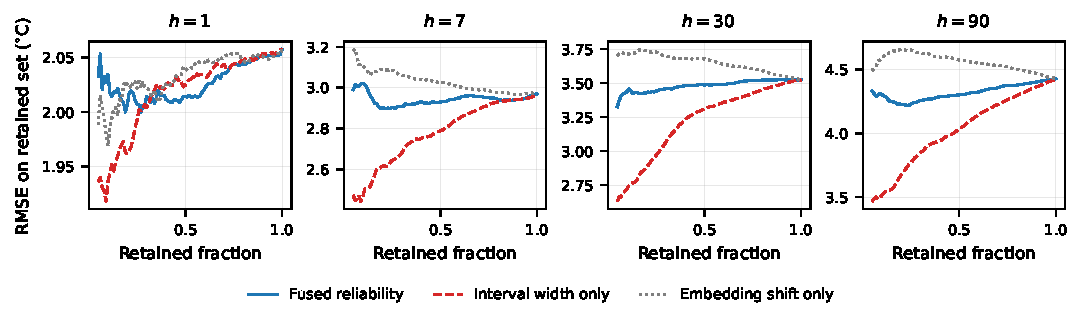
\includegraphics[width=\columnwidth]{risk_coverage.pdf}}{\fbox{\parbox{0.9\columnwidth}{\centering Risk--coverage figure will be generated from experiment outputs.}}}
\caption{Risk--coverage behaviour for selective forecasting.}
\label{fig:riskcoverage}
\end{figure}

\subsection{Ablation Study}
\todo{Report the predefined A0--A9 ablations. Remove any claimed contribution whose ablation does not show incremental and reproducible value.}

\subsection{Interpretability and Explanation Stability}
\todo{Visualize representative KAN functions and quantify stability across seeds, periods, and perturbations. Distinguish physically plausible observations from unsupported causal interpretation.}

\subsection{Robustness, Extremes, and Efficiency}
\todo{Report noise, missing-data, extreme-event, and computational experiments. Include failure cases and performance/complexity trade-offs.}

\section{Discussion}
\label{sec:discussion}

\subsection{What the Refutation Does and Does Not Show}
The results reject three specific propositions on one dataset: that this temporal KAN module improves accuracy over a budget-matched plain KAN, that fusing embedding shift with interval width yields a better reliability signal than width alone, and that the resulting score can identify forecasts that will fail. They do not show that KANs are unsuitable for climate forecasting, that shift detection is useless in general, or that selective prediction does not work. The plain KAN is a competitive model here, and width-based selection works well; what fails is the specific composition we proposed.

The generality of the refutation is nonetheless asymmetric with respect to the positive claim it replaces. Had \method{} won, a single station over a single record would have been weak evidence for a general architectural advantage. Because it loses, and loses to the ablation designed to isolate its central component, the burden shifts: a design that cannot beat its own control on a long, clean, well-understood series has not earned the presumption that it would succeed elsewhere. We report the result at this scope and state the extension to station-generalization data as unfinished work rather than as a defence.

\subsection{Why the Fusion Degrades a Working Signal}
The most instructive negative result is that the fused score is worse than one of its own inputs. Interval width carries real information about difficulty, as the width-only ablation demonstrates. The embedding-shift statistic carries little, as the shift-only ablation demonstrates. Combining them at the frozen equal weighting therefore dilutes the informative signal with an uninformative one, and the AURC penalty grows with horizon precisely where the width signal is strongest.

This suggests a methodological point that outlasts the specific design. The fusion weights were frozen at equal values because freezing was treated as sufficient protection against post-hoc tuning. Freezing an arbitrary value is not the same as choosing a defensible one: it prevents the weights from being fitted to the test set, but it does nothing to ensure they are reasonable, and it can lock in a choice that is worse than either endpoint. The correct discipline is to select such constants on the validation partition, which is legitimate and was available to us, and to freeze the selection procedure rather than the resulting number. We did not do this, and the consequence is a component that is worse than its own ablation. We report the frozen result rather than retuning, because retuning after seeing these tables would convert a pre-registered test into an exploratory one; a validation-selected weighting is the appropriate subject of a subsequent, separately pre-registered study.

\subsection{Marginal Coverage Is Not Evidence of Method Quality}
Conformal marginal coverage was the framework's most presentable number and its least meaningful one. Split conformal delivers it for any predictor under exchangeability, so reporting it as a property of \method{} would attribute to the architecture something contributed entirely by the wrapper. The joint-coverage collapse, from $0.894$ to $0.103$ across the horizon range, is the more decision-relevant quantity and points the other way. We note this because marginal coverage tables are common in the trustworthy-forecasting literature and are easy to read as validation of a method rather than of a calibration procedure.

\subsection{Interpretability versus Reliability}
KAN functions can provide inspectable nonlinear relationships, but interpretability and reliability are distinct properties, and this study separates them more sharply than intended. Any interpretability analysis of \method{} now describes a representation that is less accurate than a plain KAN at every horizon beyond one day, so the inspected functions cannot be presented as explaining superior behaviour. Stable functions may still aid scientific inspection; they are simply not evidence of forecast reliability, and the reliability measurements reported here are the relevant test of that.

\subsection{On Finding a Defect Mid-Study}
The mean-pooled readout described in Section~\ref{sec:correction} averaged encoder states over the full history window and discarded recency, leaving the model behind persistence. It was found because a pre-registered baseline comparison made the failure impossible to overlook, not because of a code review. Two aspects are worth recording. First, the defect was silent: training converged, losses looked reasonable, and every artifact validated. Only the comparison against a trivial baseline exposed it. Second, correcting it changed the code fingerprint and invalidated every completed run, which forced a full re-execution; the audit refuses to aggregate across fingerprints precisely so that this cost cannot be avoided by mixing old and new results. The correction improved the model substantially and it still loses, which is the finding reported here.

\subsection{Limitations}
Several limitations bound these conclusions. The headline evidence is a single long station record, so the results establish failure on CET rather than universal ranking; the station-generalization campaign that would test breadth is specified and not yet executed, and the multivariate protocols are frozen but unreported for lack of data access. Conformal guarantees depend on exchangeability assumptions that temporal dependence and nonstationarity strain, which is one reason joint coverage degrades. Mahalanobis-type embedding distance captures only one form of representation shift, so the shift component's poor showing is evidence against this operationalization rather than against shift-aware reliability as an idea. Selective prediction is only meaningful where abstention or escalation is operationally available. Finally, the comparison family was fixed at two comparators; a wider family would give a fuller picture of where the design sits, at the cost of multiplicity corrections that were not pre-specified.

\subsection{Reproducibility and Scientific Integrity}
Every headline number is generated from immutable, checksum-bound experiment outputs by a script that refuses to build a table from runs produced under superseded code. The claim--evidence matrix records outcomes against the evidence each claim required, including the rows now marked refuted. Failed runs, the defect and its correction, and the datasets and horizons on which the method underperforms all remain visible. This apparatus did not make the project succeed; it made it possible to know that it did not, which is the more useful of the two outcomes to be able to distinguish.

\section{Conclusion}

Two things can be wrong with a trustworthy forecasting system without any of its reported numbers looking wrong. It can ignore most of the input it is configured to read, and the score it uses to judge its own forecasts can be worse than one of the signals it is built from. This paper contributes a diagnostic for each, and a design corrected by them.

The effective-receptive-field audit is a training-free perturbation sweep that reports how much of its history a model can actually condition on, measured on the reported weights and gated on their reproducing the ledger. It found a published temporal stem admitting \robustFieldPublished{} of \robustHistory{} configured steps, a gap that no accuracy, coverage, or interpretability measurement in an earlier full campaign had surfaced. Replacing that stem with a causal dilated stack whose reach is a closed-form property of its depth, and adding an attention readout so a year of context need not pass through one final state, gives a model that reads its window and, in the paired family, is significantly better than a budget-matched plain KAN, better than the architecture it replaces at every horizon, and better than a wide-stem-only variant at \pairedDilatedWinHorizons{} and nowhere else.

Against the strongest baseline the corrected model is statistically tied: \pairedTransformerWins{} of \pairedTransformerTotal{} pairs favour it, \pairedTransformerLosses{} favours the transformer, and \pairedTransformerTied{} are inconclusive after Holm correction. We claim no accuracy advantage there and have written the generators so the tables cannot imply one.

Calibration-selected fusion replaces a frozen combination weight with a frozen selection procedure, over a grid whose endpoints are the single-component scores. The construction removes the fusion-loses-to-its-own-component failure mode outright, and it allows the data to withhold mass from an unhelpful signal: on CET the procedure put \fusionWeightLow{}--\fusionWeightHigh{} of the mass on interval width and never selected equal weights in \fusionRuns{} runs. The reliability behaviour that follows is the substance of the paper. Error detection rises from \errorAurocOne{} at one day to \errorAurocNinety{} at ninety, simultaneous joint coverage holds at \simulCoverageThirty{}--\simulCoverageNinety{} against a nominal \nominalCoverage{}, and rank correlation with realized error reaches $|\rho|=\reliabilityRhoMax{}$.

The boundaries are as much a result as the gains. Day-ahead error detection is at chance because day-ahead error on this record is irreducible from anything internal to the model. The shift term's marginal contribution to selective risk stays negligible even once its weight is fitted; what the fitting changed is that the method reaches that conclusion itself rather than requiring a refutation to establish it. The correction costs several times the training time of the cheapest neural baseline. And all of this is one station: the station-generalization protocol is frozen and unexecuted, and it is the obvious next obligation.

The general lesson concerns what reliability evidence has to be about. A configured context length is not an effective one, and only the second is a property of the model; a frozen constant is not a conservative choice when it governs how evidence is combined, and only a frozen procedure is. Both distinctions cost almost nothing to check, and in this study each of them was the difference between a system that reported reliability and one that had it.


\bibliographystyle{IEEEtran}
\bibliography{references}
\end{document}
